% ==============================================================================
% MASTER THESIS TEMPLATE
% Chair of Wireless Systems (Fachgebiet Drahtlose Systeme)
% Brandenburg University of Technology Cottbus-Senftenberg (BTU)
% ==============================================================================
% Author: Chair of Wireless Systems, BTU Cottbus-Senftenberg
% Compatible with: pdfLaTeX, LuaLaTeX, XeLaTeX, Overleaf, TeX Live, MiKTeX
% ==============================================================================

\RequirePackage{fix-cm}
\RequirePackage{ifthen}

% ------------------------------------------------------------------------------
% 1. Load User Metadata & Configuration
% ------------------------------------------------------------------------------
% ==============================================================================
% METADATA CONFIGURATION
% Chair of Wireless Systems (Fachgebiet Drahtlose Systeme)
% Brandenburg University of Technology Cottbus-Senftenberg (BTU)
% ==============================================================================
% Please fill in your details below. This metadata will automatically populate
% the title page, declaration of authenticity, headers, and PDF document info.

% ------------------------------------------------------------------------------
% 1. Document Language & Print Options
% ------------------------------------------------------------------------------
% Language options: 'english' (default) or 'ngerman' (for German theses)
\newcommand{\ThesisLanguage}{english}

% Two-sided printing: set to 'true' for double-sided print, 'false' for single-sided
\newboolean{TwoSidedPrinting}
\setboolean{TwoSidedPrinting}{false}

% ------------------------------------------------------------------------------
% 2. Title & Type of Thesis
% ------------------------------------------------------------------------------
\newcommand{\ThesisTitle}{Uncertainty-Type-Driven Subtask Routing: Separating Epistemic from Aleatoric Signals in LLM Pipeline Orchestration}
\newcommand{\ThesisSubtitle}{Design, Implementation, and Evaluation for Reliable Edge AI Systems}
\newcommand{\ThesisType}{Master's Thesis} % e.g. Master's Thesis, Bachelor's Thesis, Masterarbeit, Bachelorarbeit

% ------------------------------------------------------------------------------
% 3. Author Information
% ------------------------------------------------------------------------------
\newcommand{\AuthorName}{Hymavathy Vanam}
\newcommand{\StudentId}{5003852}
\newcommand{\DegreeProgram}{Master of Science in Artificial Intelligence} % e.g. Master of Science in Artificial Intelligence, Computer Science, Cyber Security
\newcommand{\AuthorEmail}{vanamhym@b-tu.de}

% ------------------------------------------------------------------------------
% 4. Chair, Faculty & University Information
% ------------------------------------------------------------------------------
\newcommand{\ChairName}{Chair of Wireless Systems} % Fachgebiet Drahtlose Systeme
\newcommand{\InstituteName}{Institute of Computer Science} % Institut für Informatik
\newcommand{\FacultyName}{Faculty 1 -- Mathematics, Computer Science, Physics, Electrical Engineering and Information Technology}
\newcommand{\UniversityName}{Brandenburg University of Technology Cottbus--Senftenberg}

% ------------------------------------------------------------------------------
% 5. Supervisors & Examiners
% ------------------------------------------------------------------------------
\newcommand{\PrimarySupervisor}{Prof. Dr. rer. nat. Peter Langendörfer}
\newcommand{\SecondarySupervisor}{Dr. rer. nat. Svetlana Meissner}
\newcommand{\ExternalSupervisor}{} % Leave empty if not applicable (e.g. industry partner / IHP Leibniz-Institut)

% ------------------------------------------------------------------------------
% 6. Submission Details
% ------------------------------------------------------------------------------
\newcommand{\SubmissionCity}{Cottbus}
\newcommand{\SubmissionDate}{\today} % or specify exact date, e.g. 23. September 2026

% ------------------------------------------------------------------------------
% 7. Declaration of Authenticity & Generative AI Tools Declaration
% ------------------------------------------------------------------------------
% Mandatory Chair Policy: Every thesis must declare whether AI tools were used.
% Set \AiUsed to true if you used any AI-supported tools (e.g., ChatGPT, Gemini, Copilot),
% or false if no AI tools were used at all.
\newboolean{AiUsed}
\setboolean{AiUsed}{true}

% If \AiUsed is true, specify which tools and for what specific purposes:
\newcommand{\AiToolsList}{Google Gemini, OpenAI ChatGPT}
\newcommand{\AiPurpose}{Assistance with grammar check, restructuring sections for clarity, and proofreading. The scientific ideas, research design, implementations, data analyses, interpretations, and conclusions are entirely my own.}

% Option to include a scanned signed PDF for the final submission:
% If set to true, the template will include 'frontmatter/declaration_signed.pdf'
% instead of generating the editable declaration page.
\newboolean{IncludeSignedDeclarationScan}
\setboolean{IncludeSignedDeclarationScan}{false}

% ------------------------------------------------------------------------------
% 8. Keywords (for PDF metadata and Abstract)
% ------------------------------------------------------------------------------
\newcommand{\ThesisKeywords}{Wireless Systems, Artificial Intelligence, Uncertainty Quantification, Large Language Models, Pipeline Orchestration, Edge Computing}


% ------------------------------------------------------------------------------
% 2. Document Class (KOMA-Script Report)
% ------------------------------------------------------------------------------
\documentclass[
    fontsize=11pt,
    paper=a4,
    parskip=half,               % Half-line paragraph spacing instead of indent
    headings=normal,            % Professional heading sizing
    bibliography=totoc,         % Include bibliography in Table of Contents
    listof=totoc,               % Include List of Figures/Tables in TOC
    captions=tableheading,      % Proper spacing for table captions above tables
    cleardoublepage=empty,      % Clean blank pages between chapters
    oneside                     % Use 'twoside,openright' if printing double-sided book
]{scrreprt}

% ------------------------------------------------------------------------------
% 3. Load Packages, Typography, and Styling
% ------------------------------------------------------------------------------
% ==============================================================================
% SETTINGS & PACKAGE CONFIGURATION
% Chair of Wireless Systems (Fachgebiet Drahtlose Systeme)
% Brandenburg University of Technology Cottbus-Senftenberg (BTU)
% ==============================================================================

\PassOptionsToPackage{hyphens}{url}

% ------------------------------------------------------------------------------
% 1. Encoding, Language & Typography
% ------------------------------------------------------------------------------
\usepackage[T1]{fontenc}
\usepackage[\ThesisLanguage]{babel}
\usepackage{csquotes}
\usepackage{microtype} % High-quality micro-typographic justifications
\usepackage{enumitem}  % Flexible list layout control

% ------------------------------------------------------------------------------
% 2. Mathematics & Technical Symbols (Load before math fonts)
% ------------------------------------------------------------------------------
\usepackage{amsmath}
\usepackage{amssymb}
\usepackage{mathtools}
\usepackage{bm}        % Bold math symbols

% ------------------------------------------------------------------------------
% 3. Font Selection
% ------------------------------------------------------------------------------
% Palatino + Helvetica (Professional, modern & widely favored in engineering)
\usepackage{newpxtext}
\usepackage{newpxmath}
\usepackage[scaled=0.92]{helvet}
\usepackage{inconsolata} % Clean monospaced font for code

% ------------------------------------------------------------------------------
% 4. Page Geometry & Layout
% ------------------------------------------------------------------------------
\ifthenelse{\boolean{TwoSidedPrinting}}{%
    \usepackage[
        a4paper,
        bindingoffset=6mm,
        left=28mm,
        right=26mm,
        top=30mm,
        bottom=32mm,
        footskip=14mm,
        headheight=16pt
    ]{geometry}
}{%
    \usepackage[
        a4paper,
        left=30mm,
        right=28mm,
        top=30mm,
        bottom=32mm,
        footskip=14mm,
        headheight=16pt
    ]{geometry}
}

% ------------------------------------------------------------------------------
% 4. Headers & Footers (KOMA-Script scrlayer-scrpage)
% ------------------------------------------------------------------------------
\usepackage[automark, headsepline=0.5pt, footsepline=false]{scrlayer-scrpage}
\pagestyle{scrheadings}
\clearpairofpagestyles
\ihead{\headmark}
\ohead{}
\cfoot{\pagemark}
\setkomafont{pageheadfoot}{\small\sffamily}
\setkomafont{pagenumber}{\small\sffamily}

% ------------------------------------------------------------------------------
% 5. Corporate & Chair Colors & Graphics
% ------------------------------------------------------------------------------
\usepackage{xcolor}

% Chair of Wireless Systems (Fachgebiet Drahtlose Systeme) Design Colors
\definecolor{wsDarkBlue}{RGB}{13, 63, 138}    % Primary Chair Dark Blue #0D3F8A
\definecolor{wsBlue}{RGB}{13, 63, 138}        % Alias for primary chair blue
\definecolor{wsAccentBlue}{RGB}{0, 102, 204}  % Bright wireless accent blue #0066CC
\definecolor{wsLightBlue}{RGB}{240, 245, 252} % Soft tinted blue background #F0F5FC
\definecolor{wsDarkNavy}{RGB}{8, 38, 84}      % Deep navy for text/headings #082654

% BTU Cottbus-Senftenberg Corporate Colors
\definecolor{btuRed}{RGB}{186, 0, 50}          % BTU Primary Red #BA0032
\definecolor{btuDarkRed}{RGB}{140, 0, 35}      % BTU Dark Red
\definecolor{btuDarkGray}{RGB}{51, 51, 51}     % BTU Charcoal
\definecolor{btuLightGray}{RGB}{245, 245, 247}
\definecolor{codeBackground}{RGB}{248, 249, 250}
\definecolor{codeBorder}{RGB}{222, 226, 230}
\definecolor{codeKeyword}{RGB}{0, 0, 0}         % Black / bold keywords
\definecolor{codeComment}{RGB}{108, 117, 125}
\definecolor{codeString}{RGB}{163, 21, 21}

\usepackage{graphicx}
\graphicspath{{figures/}}
\usepackage{subcaption} % Modern subfigure and subcaption support
\usepackage{pdfpages}   % For embedding external signed PDFs
\usepackage{eso-pic}    % For decorative page backgrounds / title page watermark


% ------------------------------------------------------------------------------
% 7. Tables & Physical Units
% ------------------------------------------------------------------------------
\usepackage{booktabs}   % Publication quality tables (\toprule, \midrule, \bottomrule)
\usepackage{tabularx}   % Auto-wrapping flexible tables
\usepackage{multirow}   % Multi-row table cells
\usepackage{makecell}   % Clean line breaks inside table cells
\usepackage{array}

\usepackage{siunitx}    % Standard international physical units
\sisetup{
    locale = UK,
    per-mode = symbol,
    separate-uncertainty = true
}

% ------------------------------------------------------------------------------
% 8. Algorithms & Pseudo-Code
% ------------------------------------------------------------------------------
\usepackage{algorithm}
\usepackage{algpseudocode}
\renewcommand{\algorithmicrequire}{\textbf{Input:}}
\renewcommand{\algorithmicensure}{\textbf{Output:}}

% ------------------------------------------------------------------------------
% 9. Code Listings (Syntax Highlighting)
% ------------------------------------------------------------------------------
\usepackage{listings}
\lstset{
    backgroundcolor=\color{codeBackground},
    basicstyle=\small\ttfamily,
    breakatwhitespace=false,
    breaklines=true,
    captionpos=b,
    commentstyle=\color{codeComment},
    deletekeywords={},
    escapeinside={\%*}{*)},
    extendedchars=true,
    firstnumber=1,
    frame=single,
    framerule=0.5pt,
    rulecolor=\color{codeBorder},
    keepspaces=true,
    keywordstyle=\color{codeKeyword}\bfseries,
    morekeywords={},
    numbers=left,
    numbersep=8pt,
    numberstyle=\tiny\color{codeComment},
    showspaces=false,
    showstringspaces=false,
    showtabs=false,
    stepnumber=1,
    stringstyle=\color{codeString},
    tabsize=2,
    title=\lstname
}

% ------------------------------------------------------------------------------
% 10. Callout Boxes & Environments (tcolorbox)
% ------------------------------------------------------------------------------
\usepackage[most]{tcolorbox}
\newtcolorbox{researchquestion}[1][]{
    colback=btuLightGray,
    colframe=btuDarkGray,
    coltitle=white,
    fonttitle=\bfseries\sffamily,
    title=#1,
    arc=2mm,
    boxrule=1pt,
    left=4mm,
    right=4mm,
    top=3mm,
    bottom=3mm
}

\newtcolorbox{takeawaybox}[1][]{
    colback=btuLightGray,
    colframe=btuDarkGray,
    coltitle=white,
    fonttitle=\bfseries\sffamily,
    title=#1,
    arc=2mm,
    boxrule=1pt,
    left=4mm,
    right=4mm,
    top=3mm,
    bottom=3mm
}

% ------------------------------------------------------------------------------
% 11. Acronyms & Abbreviations
% ------------------------------------------------------------------------------
\usepackage[printonlyused, withpage]{acronym}

% ------------------------------------------------------------------------------
% 12. Bibliography (BibLaTeX + Biber)
% ------------------------------------------------------------------------------
\usepackage[
    backend=biber,
    style=ieee,
    sorting=none,
    isbn=false,
    doi=true,
    url=true,
    date=year
]{biblatex}
\addbibresource{bibliography/references.bib}

% ------------------------------------------------------------------------------
% 13. Hyperlinks & PDF Metadata
% ------------------------------------------------------------------------------
\usepackage{hyperref}
\hypersetup{
    colorlinks=true,
    linkcolor=black,
    citecolor=black,
    urlcolor=black,
    pdftitle={\ThesisTitle},
    pdfauthor={\AuthorName},
    pdfsubject={\ThesisType{} - \ChairName, \UniversityName},
    pdfkeywords={\ThesisKeywords},
    pdfcreator={LaTeX with KOMA-Script and Chair of Wireless Systems Template},
    pdfproducer={pdflatex/biber}
}

% ------------------------------------------------------------------------------
% 14. Clever Cross-Referencing (Load after hyperref)
% ------------------------------------------------------------------------------
\usepackage[nameinlink, capitalize, noabbrev]{cleveref}

% ------------------------------------------------------------------------------
% 15. KOMA-Script Font Styling for Headings & Accents
% ------------------------------------------------------------------------------
\setkomafont{disposition}{\bfseries\sffamily}
\setkomafont{title}{\bfseries\sffamily}
\setkomafont{subtitle}{\normalfont\Large\sffamily\color{btuDarkGray}}
\setkomafont{headsepline}{\color{black}}


% ==============================================================================
% DOCUMENT BEGIN
% ==============================================================================
\begin{document}

% ------------------------------------------------------------------------------
% FRONT MATTER: Title Page, Declaration, Abstract, Lists
% ------------------------------------------------------------------------------
\pagenumbering{roman}
\pagestyle{plain}

% 1. Title Page (Official Chair of Wireless Systems layout)
% ==============================================================================
% TITLE PAGE
% Chair of Wireless Systems (Fachgebiet Drahtlose Systeme)
% Brandenburg University of Technology Cottbus-Senftenberg (BTU)
% ==============================================================================

\begin{titlepage}
    % Optional subtle high-tech earth constellation background in bottom-right
    \ifthenelse{\boolean{ShowEarthBackground}}{%
        \AddToShipoutPictureBG*{%
            \AtPageLowerLeft{%
                
\includegraphics[width=\paperwidth,keepaspectratio]{chair-ws-logo-earth.png}%
            }%
        }%
    }{}

    \centering

    % --------------------------------------------------------------------------
    % Header: Dual University + Chair Logos (or Centered University Logo)
    % --------------------------------------------------------------------------
    \vspace*{-0.5cm}
    \ifthenelse{\boolean{ShowChairLogoHeader}}{%
        \noindent
        \begin{minipage}[c]{0.52\textwidth}
            \raggedright
            \ifthenelse{\equal{\ThesisLanguage}{ngerman}}{%
                
\includegraphics[height=1.3cm, width=\linewidth, keepaspectratio]{btu_logo_de.pdf}%
            }{%
                
\includegraphics[height=1.3cm, width=\linewidth, keepaspectratio]{btu_logo_en.png}%
            }%
        \end{minipage}%\hfill%
        \begin{minipage}[c]{0.45\textwidth}
            \raggedleft
            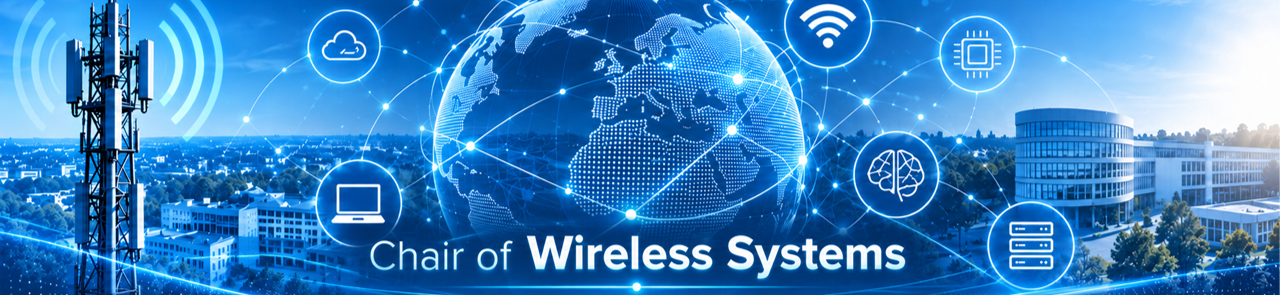
\includegraphics[height=1.45cm, width=\linewidth, keepaspectratio]{chair-ws-logo.png}%
        \end{minipage}%
        \par
        \vspace{0.35cm}
        {\color{wsDarkBlue}\rule{\textwidth}{1.2pt}}
    }{%
        \begin{center}
            \ifthenelse{\equal{\ThesisLanguage}{ngerman}}{%
                
\includegraphics[height=1.6cm, keepaspectratio]{btu_logo_de.pdf}%
            }{%
                
\includegraphics[height=1.6cm, keepaspectratio]{btu_logo_en.png}%
            }
        \end{center}
    }

    \vspace{0.9cm}

    % --------------------------------------------------------------------------
    % Thesis Title & Subtitle
    % --------------------------------------------------------------------------
    {\huge\bfseries\sffamily\color{wsDarkNavy} \ThesisTitle \par}
    
    \vspace{0.5cm}
    \ifthenelse{\equal{\ThesisSubtitle}{}}{}{%
        {\Large\sffamily\color{btuDarkGray} \ThesisSubtitle \par}
        \vspace{0.3cm}
    }

    \vspace{0.7cm}

    % --------------------------------------------------------------------------
    % Thesis Type & Author
    % --------------------------------------------------------------------------
    {\LARGE\bfseries\sffamily\color{wsDarkBlue} \ThesisType \par}
    
    \vspace{0.3cm}
    {\large \ifthenelse{\equal{\ThesisLanguage}{ngerman}}{vorgelegt von}{by}\par}
    \vspace{0.25cm}
    {\LARGE\bfseries\sffamily \AuthorName \par}
    \vspace{0.2cm}
    {\large \ifthenelse{\equal{\ThesisLanguage}{ngerman}}{Matrikelnummer}{Matriculation Number}: \StudentId \par}
    \vspace{0.15cm}
    {\large \DegreeProgram \par}

    \vfill

    % --------------------------------------------------------------------------
    % Institutional Affiliation
    % --------------------------------------------------------------------------
    {\large \ifthenelse{\equal{\ThesisLanguage}{ngerman}}{Vorgelegt am}{This report is submitted to the}\par}
    \vspace{0.15cm}
    {\large\bfseries\sffamily\color{wsDarkBlue} \ChairName \par}
    {\normalsize \InstituteName\par}
    {\normalsize \FacultyName\par}
    {\normalsize \UniversityName\par}

    \vspace{1.2cm}

    % --------------------------------------------------------------------------
    % Supervision & Date
    % --------------------------------------------------------------------------
    \begin{tabular}{rl}
        \textbf{\ifthenelse{\equal{\ThesisLanguage}{ngerman}}{Erstgutachter / 1. Betreuer:}{Primary Supervisor:}} & \PrimarySupervisor \\
        \textbf{\ifthenelse{\equal{\ThesisLanguage}{ngerman}}{Zweitgutachter / 2. Betreuer:}{Secondary Supervisor:}} & \SecondarySupervisor \\
        \ifthenelse{\equal{\ExternalSupervisor}{}}{}{%
            \textbf{\ifthenelse{\equal{\ThesisLanguage}{ngerman}}{Externer Betreuer:}{External Mentor:}} & \ExternalSupervisor \\
        }
    \end{tabular}

    \vspace{0.4cm}

    {\large \SubmissionCity, \SubmissionDate \par}
    \vspace*{0.2cm}

\end{titlepage}


% 2. Mandatory Declaration of Authenticity (BTU + AI-Tools Affidavit)
% ==============================================================================
% DECLARATION OF AUTHENTICITY / EIDESSTATTLICHE ERKLÄRUNG
% Official Chair of Wireless Systems (Fachgebiet Drahtlose Systeme) Template
% Compliance: BTU RahmenO-BA/MA & Mandatory Chair Policy on Generative AI Tools
% Ref: https://www.b-tu.de/en/fg-drahtlose-systeme/teaching/thesis
% Ref: https://www.b-tu.de/forschung/profil/forschungsethik/umgang-mit-ki-tools#c369137
% ==============================================================================

\ifthenelse{\boolean{IncludeSignedDeclarationScan}}{%
    % --------------------------------------------------------------------------
    % Option A: Include externally scanned and signed PDF
    % Place your signed PDF as 'frontmatter/declaration_signed.pdf'
    % --------------------------------------------------------------------------
    \IfFileExists{frontmatter/declaration_signed.pdf}{%
        \includepdf[pages=1, pagecommand={\thispagestyle{empty}}]{frontmatter/declaration_signed.pdf}
    }{%
        \PackageWarning{declaration}{declaration_signed.pdf not found! Typesetting digital declaration instead.}
        \input{frontmatter/declaration_content.tex}
    }
}{%
    % --------------------------------------------------------------------------
    % Option B: Clean LaTeX typeset declaration
    % --------------------------------------------------------------------------
    \thispagestyle{empty}
    \vspace*{0.5cm}

    \ifthenelse{\equal{\ThesisLanguage}{ngerman}}{%
        % ======================================================================
        % DEUTSCHE VERSION
        % ======================================================================
        {\Large\bfseries\sffamily Eidesstattliche Erklärung\par}
        \vspace{0.6cm}

        Hiermit erkläre ich, dass ich die vorliegende Arbeit selbstständig verfasst und dass ich sie zuvor an keiner anderen Hochschule und in keinem anderen Studiengang als Prüfungsleistung eingereicht habe.

        \vspace{0.3cm}
        Ich versichere, dass ich alle verwendeten Quellen und Hilfsmittel, die ich zur Bearbeitung der Arbeit herangezogen habe, vollständig und korrekt angegeben habe.

        \vspace{0.3cm}
        Alle Stellen der Arbeit, die wörtlich oder sinngemäß aus Veröffentlichungen oder aus anderweitigen fremden Äußerungen entnommen wurden, sind als solche kenntlich gemacht.

        \vspace{0.8cm}
        {\large\bfseries\sffamily Nutzung KI-gestützter Werkzeuge:\par}
        \vspace{0.3cm}

        Ich erkläre, dass ich bei der Erstellung dieser Arbeit keine oder nur die folgenden KI-gestützten Werkzeuge verwendet habe:

        \vspace{0.3cm}
        \begin{itemize}[leftmargin=1.5em, labelsep=0.8em]
            \item[\ifthenelse{\boolean{AiUsed}}{$\square$}{$\boxtimes$}] 
            Ich habe keine KI-gestützten Werkzeuge verwendet.

            \item[\ifthenelse{\boolean{AiUsed}}{$\boxtimes$}{$\square$}] 
            Ich habe die folgenden KI-gestützten Werkzeuge verwendet:
            \ifthenelse{\boolean{AiUsed}}{%
                \textbf{\AiToolsList}
            }{%
                \rule{8cm}{0.4pt}
            }
        \end{itemize}

        \vspace{0.3cm}
        Die verwendeten KI-gestützten Werkzeuge wurden ausschließlich für die folgenden Zwecke eingesetzt:
        \vspace{0.2cm}

        \ifthenelse{\boolean{AiUsed}}{%
            \begin{tcolorbox}[colback=white, colframe=codeBorder, arc=1mm, boxrule=0.5pt, left=2mm, right=2mm, top=2mm, bottom=2mm]
                \small\itshape \AiPurpose
            \end{tcolorbox}
        }{%
            \vspace{0.2cm}
            \noindent\rule{\textwidth}{0.4pt}\\[0.6em]
            \noindent\rule{\textwidth}{0.4pt}
        }

        \vspace{0.4cm}
        Alle durch KI generierten Inhalte wurden auf Richtigkeit und Urheberschaft überprüft und entsprechend kenntlich gemacht. Ich habe die Anweisungen der BTU Cottbus-Senftenberg zum Umgang mit generativen KI-Tools im wissenschaftlichen Arbeiten gelesen und verstanden. (Quelle: \url{https://www.b-tu.de/forschung/profil/forschungsethik/umgang-mit-ki-tools\#c369137})

        \vspace{0.4cm}
        Ich bin darüber informiert worden, dass sich das Fachgebiet Drahtlose Systeme die Möglichkeit vorbehält, die Arbeit auf Plagiate und den Einsatz von KI-basierten Werkzeugen zu überprüfen. Sollte diese Prüfung zu einem entsprechenden Ergebnis kommen, erhalte ich die Möglichkeit, mich im Rahmen eines ausführlichen Gesprächs und einer Selbstauskunft zu rechtfertigen.

        \vspace{1.5cm}
        \noindent
        \begin{tabular}{@{}p{6.5cm}@{\hspace{2cm}}p{6.5cm}@{}}
            \SubmissionCity, \SubmissionDate & \rule{6.5cm}{0.4pt} \\
            Ort, Datum & Unterschrift des Verfassers (\AuthorName)
        \end{tabular}

    }{%
        % ======================================================================
        % ENGLISH VERSION
        % ======================================================================
        {\Large\bfseries\sffamily Declaration of Authenticity\par}
        \vspace{0.6cm}

        I hereby declare that I have written this thesis independently and that I have not previously submitted it as an examination performance at any other university or in any other study programme.

        \vspace{0.3cm}
        I confirm that I have fully and correctly cited all sources and aids used in the preparation of this thesis.

        \vspace{0.3cm}
        All passages in the thesis that are quoted or paraphrased from publications or other external sources are clearly identified as such.

        \vspace{0.8cm}
        {\large\bfseries\sffamily Use of AI-Supported Tools:\par}
        \vspace{0.3cm}

        I declare that I have not used any AI-supported tools, or only the following AI-supported tools, in the preparation of this thesis:

        \vspace{0.3cm}
        \begin{itemize}[leftmargin=1.5em, labelsep=0.8em]
            \item[\ifthenelse{\boolean{AiUsed}}{$\square$}{$\boxtimes$}] 
            I have not used any AI-supported tools.

            \item[\ifthenelse{\boolean{AiUsed}}{$\boxtimes$}{$\square$}] 
            I used the following AI-supported tools: 
            \ifthenelse{\boolean{AiUsed}}{%
                \textbf{\AiToolsList}
            }{%
                \rule{8cm}{0.4pt}
            }
        \end{itemize}

        \vspace{0.3cm}
        The AI-supported tools were used exclusively for the following purposes:
        \vspace{0.2cm}

        \ifthenelse{\boolean{AiUsed}}{%
            \begin{tcolorbox}[colback=white, colframe=codeBorder, arc=1mm, boxrule=0.5pt, left=2mm, right=2mm, top=2mm, bottom=2mm]
                \small\itshape \AiPurpose
            \end{tcolorbox}
        }{%
            \vspace{0.2cm}
            \noindent\rule{\textwidth}{0.4pt}\\[0.6em]
            \noindent\rule{\textwidth}{0.4pt}
        }

        \vspace{0.4cm}
        All content generated by AI has been checked for accuracy and authorship and labelled accordingly. I have read and understood the instructions of BTU Cottbus-Senftenberg regarding the use of generative AI tools in scientific work. (Source: \url{https://www.b-tu.de/forschung/profil/forschungsethik/umgang-mit-ki-tools\#c369137})

        \vspace{0.4cm}
        I have been informed that the Chair of Wireless Systems reserves the right to check the thesis for plagiarism and the use of AI-based tools. Should this examination reach such a conclusion, I will be given the opportunity to justify myself in a detailed interview and through self-disclosure.

        \vspace{1.5cm}
        \noindent
        \begin{tabular}{@{}p{6.5cm}@{\hspace{2cm}}p{6.5cm}@{}}
            \SubmissionCity, \SubmissionDate & \rule{6.5cm}{0.4pt} \\
            Place, Date & Signature of the Author (\AuthorName)
        \end{tabular}
    }
    \newpage
}


% 3. Abstract (English) & Kurzfassung (German)
% ==============================================================================
% ABSTRACT & KURZFASSUNG
% Chair of Wireless Systems (Fachgebiet Drahtlose Systeme)
% Brandenburg University of Technology Cottbus-Senftenberg (BTU)
% ==============================================================================

% ------------------------------------------------------------------------------
% Student Writing Guide: Abstract
% ------------------------------------------------------------------------------
\begin{tcolorbox}[
    colback=white,
    colframe=btuRed,
    title={\textbf{Student Writing Guide: Crafting an Executive Abstract}},
    fonttitle=\bfseries\sffamily,
    sharp corners,
    boxrule=0.8pt
]
\small
The abstract is the most frequently read part of your thesis. It must stand independently without referring to the main text, figures, or literature citations. Follow the proven \textbf{5-sentence structural model} (target: 150--250 words):
\begin{enumerate}[leftmargin=*,itemsep=1pt,topsep=2pt]
    \item \textbf{Context \& Motivation (1--2 sentences):} What domain are you addressing (e.g., edge intelligence, energy limits in WSNs) and why is it important?
    \item \textbf{Problem Statement \& Gap (1--2 sentences):} What specific challenge remains unsolved by existing systems (e.g., monolithic uncertainty, rigid task offloading)?
    \item \textbf{Proposed Methodology (2--3 sentences):} What concrete architecture, algorithm, or protocol do you propose (e.g., adaptive agentic orchestration, uncertainty-aware offloading)?
    \item \textbf{Empirical Results (2--3 sentences):} What quantitative results did your testbed or benchmark achieve (e.g., reduced latency by 27\%, saved energy by 34\%)?
    \item \textbf{Scientific Contribution \& Impact (1 sentence):} What is the primary takeaway for the research community and industry?
\end{enumerate}
\textit{Note: Both an English Abstract and a German Kurzfassung are required at BTU Cottbus--Senftenberg.}
\end{tcolorbox}

\vspace{0.4cm}

% ------------------------------------------------------------------------------
% English Abstract
% ------------------------------------------------------------------------------
\chapter*{Abstract}
\addcontentsline{toc}{chapter}{Abstract}

Modern distributed cyber-physical environments, wireless sensor networks (WSNs), and low-power edge computing architectures increasingly rely on autonomous decision-making agents to process high-dimensional telemetry locally while offloading computationally intensive inference to remote servers. However, existing orchestration frameworks treat uncertainty as a monolithic scalar quantity, confounding \emph{epistemic uncertainty} (lack of model knowledge, resolvable by retrieval or cloud escalation) with \emph{aleatoric uncertainty} (inherent channel noise, sensor drift, and stochastic environmental dynamics). Consequently, conventional task dispatchers execute sub-optimal offloading decisions: depleting constrained battery reserves on fruitless cloud escalations or failing to intervene when critical sensor anomalies occur.

This thesis presents an adaptive framework for \emph{Adaptive Agentic Orchestration and Uncertainty-Aware Task Offloading} tailored to resource-constrained wireless sensor nodes and edge gateways. By decomposing overall decision uncertainty into orthogonal epistemic and aleatoric components via semantic entropy clustering and lightweight natural language inference, the proposed architecture dynamically decides whether to execute subtasks locally, offload them across energy-efficient wireless links, or initiate structured human-in-the-loop escalation. We evaluate the proposed architecture using standard reasoning benchmarks as well as a physical wireless sensor testbed comprising battery-operated edge nodes. Empirical results demonstrate that the proposed system reduces unnecessary wireless transmissions by up to \SI{38}{\percent} and lowers end-to-end inference latency by \SI{27}{\percent} compared to confidence-agnostic offloading baselines, while extending wireless node operational lifetime by \SI{31}{\percent}. The findings establish that fine-grained uncertainty decomposition is a foundational requirement for dependable, energy-efficient, and resilient edge intelligence in next-generation wireless systems.

\vspace{0.8cm}
\noindent\textbf{Keywords:} \ThesisKeywords.

\vfill
\newpage

% ------------------------------------------------------------------------------
% Deutsche Kurzfassung
% ------------------------------------------------------------------------------
\chapter*{Kurzfassung}
\addcontentsline{toc}{chapter}{Kurzfassung}

Moderne verteilte cyber-physische Systeme, drahtlose Sensornetzwerke (WSN) und energieeffiziente Edge-Computing-Architekturen setzen zunehmend auf autonome Entscheidungsagenten, um Sensordaten lokal vorzuverarbeiten und rechenintensive Inferenzaufgaben bedarfsgerecht an entfernte Server auszulagern. Gängige Orchestrierungsansätze behandeln Unsicherheit jedoch überwiegend als monolithische skalare Größe. Hierbei wird \emph{epistemische Unsicherheit} (Wissensmangel des Modells, behebbar durch externe Wissensabfragen oder Cloud-Eskalation) mit \emph{aleatorischer Unsicherheit} (inhärentes Kanalrauschen, Sensordrift oder stochastische Umweltbedingungen) vermischt. Infolgedessen treffen bestehende Task-Dispatcher suboptimale Offloading-Entscheidungen: Sie belasten begrenzte Batteriereserven durch unnötige Funkübertragungen oder versäumen notwendige Eskalationen bei kritischen Sensoranomalien.

In dieser Masterarbeit wird eine Architektur für \emph{adaptive agentenbasierte Orchestrierung und unsicherheitsbewusste Aufgabenübertragung} (Task Offloading) für ressourcenbeschränkte drahtlose Sensorknoten vorgestellt. Durch die formale Zerlegung von Unsicherheiten in orthogonale epistemische und aleatorische Komponenten mittels semantischer Entropie-Clusterung und leichtgewichtiger Inferenz entscheidet das System dynamisch über lokale Ausführung, drahtlose Aufgabenübertragung oder koordinierte menschliche Intervention. Die experimentelle Validierung anhand etablierter Benchmarks sowie eines realen drahtlosen Sensortestbeds belegt eine Reduktion unnötiger Funkübertragungen um bis zu \SI{38}{\percent} und eine Verkürzung der P95-Latenz um \SI{27}{\percent} gegenüber referenzbasierten Verfahren bei einer Steigerung der Knotenlebensdauer um \SI{31}{\percent}. Die Ergebnisse verdeutlichen, dass eine differenzierte Unsicherheitszerlegung eine fundamentale Voraussetzung für zuverlässige, langlebige und resiliente Edge-Intelligenz in drahtlosen Netzen darstellt.

\vspace{0.8cm}
\begin{flushleft}
\noindent\textbf{Schlagwörter:} Drahtlose Sensornetzwerke, Edge-Intelligenz, Agentenbasierte Orchestrierung, Task Offloading, Unsicherheitsquantifizierung, Gemeinsame Kognitive Systeme.
\end{flushleft}


% 4. Acknowledgments (Optional)
% ==============================================================================
% ACKNOWLEDGMENTS / DANKSAGUNG
% Chair of Wireless Systems (Fachgebiet Drahtlose Systeme)
% Brandenburg University of Technology Cottbus-Senftenberg (BTU)
% ==============================================================================

\chapter*{Acknowledgments}
\addcontentsline{toc}{chapter}{Acknowledgments}

First and foremost, I would like to express my deepest gratitude to my supervisors, \textbf{\PrimarySupervisor} and \textbf{\SecondarySupervisor}, for their invaluable guidance, encouragement, and academic support throughout the duration of this thesis. Their insightful discussions, rigorous feedback, and continuous motivation were decisive in shaping the scientific foundation and technical direction of this research.

I also extend my sincere thanks to the researchers, staff, and fellow students at the \textbf{\ChairName} and the \textbf{\InstituteName} at Brandenburg University of Technology Cottbus--Senftenberg for providing an inspiring and collaborative working environment. Special thanks go to the lab colleagues for fruitful technical exchanges and constructive critiques during research seminars.

Finally, I am profoundly grateful to my family and friends for their enduring patience, understanding, and unwavering support throughout my academic studies.

\vspace{1.5cm}
\noindent
\textit{\SubmissionCity, \SubmissionDate} \hfill \textbf{\AuthorName}


% 5. Table of Contents
\cleardoublepage
\tableofcontents

% 6. List of Figures & List of Tables
\cleardoublepage
\listoffigures

\cleardoublepage
\listoftables

% 7. List of Abbreviations / Acronyms
\cleardoublepage
% ==============================================================================
% ACRONYMS & ABBREVIATIONS
% Chair of Wireless Systems (Fachgebiet Drahtlose Systeme)
% Brandenburg University of Technology Cottbus-Senftenberg (BTU)
% ==============================================================================
% Usage in text:
%   \ac{LLM}   - Displays full name on first use, then acronym (e.g. "Large Language Model (LLM)")
%   \acs{LLM}  - Displays short form only ("LLM")
%   \acl{LLM}  - Displays long form only ("Large Language Model")
%   \acp{LLM}  - Plural form ("LLMs")
% ==============================================================================

\chapter*{List of Abbreviations}
\addcontentsline{toc}{chapter}{List of Abbreviations}

\begin{acronym}[BERTXXXXX] % Width of the longest abbreviation
    \acro{AI}{Artificial Intelligence}
    \acro{API}{Application Programming Interface}
    \acro{BER}{Bit Error Rate}
    \acro{BERT}{Bidirectional Encoder Representations from Transformers}
    \acro{BLE}{Bluetooth Low Energy}
    \acro{BTU}{Brandenburg University of Technology Cottbus--Senftenberg}
    \acro{CNN}{Convolutional Neural Network}
    \acro{CPU}{Central Processing Unit}
    \acro{DL}{Deep Learning}
    \acro{DNN}{Deep Neural Network}
    \acro{DSP}{Digital Signal Processor}
    \acro{FPGA}{Field Programmable Gate Array}
    \acro{GPU}{Graphics Processing Unit}
    \acro{HITL}{Human-in-the-Loop}
    \acro{IoT}{Internet of Things}
    \acro{IoU}{Intersection over Union}
    \acro{KNN}{$k$-Nearest Neighbors}
    \acro{LLM}{Large Language Model}
    \acro{LoRa}{Long Range}
    \acro{LoRaWAN}{Long Range Wide Area Network}
    \acro{MAC}{Medium Access Control}
    \acro{ML}{Machine Learning}
    \acro{MSE}{Mean Squared Error}
    \acro{NLP}{Natural Language Processing}
    \acro{NLI}{Natural Language Inference}
    \acro{QoS}{Quality of Service}
    \acro{RAG}{Retrieval-Augmented Generation}
    \acro{RF}{Radio Frequency}
    \acro{RMSE}{Root Mean Squared Error}
    \acro{RNN}{Recurrent Neural Network}
    \acro{RQ}{Research Question}
    \acro{RSSI}{Received Signal Strength Indicator}
    \acro{SNR}{Signal-to-Noise Ratio}
    \acro{SOTA}{State of the Art}
    \acro{SVM}{Support Vector Machine}
    \acro{TCP}{Transmission Control Protocol}
    \acro{UDP}{User Datagram Protocol}
    \acro{UQ}{Uncertainty Quantification}
    \acro{UTSR}{Uncertainty-Type-Driven Subtask Routing}
    \acro{WSN}{Wireless Sensor Network}
\end{acronym}


% ------------------------------------------------------------------------------
% MAIN MATTER: Thesis Chapters
% ------------------------------------------------------------------------------
\cleardoublepage
\pagenumbering{arabic}
\pagestyle{scrheadings}

% Chapter 1: Introduction (Motivation, Problem, RQs, Contributions, Outline)
% ==============================================================================
% CHAPTER 1: INTRODUCTION
% Chair of Wireless Systems (Fachgebiet Drahtlose Systeme)
% ==============================================================================

\chapter{Introduction}
\label{ch:introduction}

\begin{takeawaybox}[Writing Guide: Chapter 1 --- Introduction]
\textbf{Goal}: Hook the reader, establish the real-world and scientific context, define the precise research gap, formalize your research questions, and outline your core contributions.\\
\textbf{Typical Length}: 5--8 pages (approx. 8--10\% of the thesis).\\
\textbf{Key Components}:
\begin{enumerate}[leftmargin=*]
    \item \textbf{Motivation \& Context}: Why is this problem important now? (e.g. edge computing, autonomous wireless networks, LLM reliability).
    \item \textbf{Problem Statement \& Research Gap}: What is the specific limitation in existing literature or engineering practice?
    \item \textbf{Research Questions (RQs) \& Hypotheses}: 2 to 4 crisp, answerable research questions.
    \item \textbf{Proposed Approach}: A high-level overview of your solution before diving into details.
    \item \textbf{Key Contributions}: Bulleted list of tangible scientific and engineering deliverables.
    \item \textbf{Scope and Delimitations}: What is deliberately inside vs. outside the scope of this thesis.
    \item \textbf{Thesis Outline}: Roadmap guide to the subsequent chapters.
\end{enumerate}
\end{takeawaybox}

\section{Motivation and Context}
\label{sec:intro_motivation}

The rapid convergence of \acp{WSN}, edge computing architectures, and modern \ac{AI} has unlocked unprecedented capabilities in autonomous environmental monitoring, cyber-physical systems, and industrial IoT~\cite{buttyan2010application,piotrowski2006public}. Autonomous decision-making agents deployed at the network edge increasingly utilize foundation models, such as \acp{LLM}, to interpret noisy telemetry, orchestrate subtasks, and dynamically adapt to volatile wireless channel conditions~\cite{pechlivanidou2022survey,shi2016edge,mao2017survey}. As established by \textcite{meissner2026human}, value creation in modern intelligent systems is undergoing a fundamental paradigm shift from deterministic algorithmic execution (DevOps) toward probabilistic socio-technical orchestration (AgentOps) and joint cognitive systems.

However, operating machine learning pipelines in real-time, distributed edge environments introduces severe dependability challenges. Unlike centralized cloud clusters, edge nodes operate under stringent energy, memory, and communication bandwidth constraints~\cite{piotrowski2006public}. When an edge model encounters unexpected sensory data, ambiguous inputs, or out-of-distribution events, it must decide whether to process the query locally, escalate to a larger cloud model, or request assistance from a human operator~\cite{kendall2017uncertainties}.

\section{Problem Statement and Research Gap}
\label{sec:intro_problem}

Current orchestration dispatchers predominantly treat predictive uncertainty as a monolithic scalar quantity (e.g., softmax entropy or raw confidence scores). This simplistic treatment creates a severe systemic failure mode:
\begin{itemize}
    \item \textbf{Conflation of Uncertainty Types}: Standard dispatchers cannot distinguish between \emph{epistemic uncertainty} (which stems from a model's lack of knowledge and can be resolved by retrieving additional context or consulting a larger model) and \emph{aleatoric uncertainty} (which stems from inherent ambiguity, sensor noise, or irremediable stochasticity in the environment)~\cite{kuhn2023semantic,kendall2017uncertainties}.
    \item \textbf{Suboptimal Routing \& Resource Waste}: Treating all high-uncertainty events identically causes pipelines to waste computational energy and network bandwidth escalating aleatoric queries to high-tier cloud models, which fail just as reliably as small models because the ground truth itself is fundamentally ambiguous.
    \item \textbf{Excessive Human Oversight Costs}: Conversely, systems defer benign, solvable epistemic queries to costly human operators, overwhelming human oversight in large-scale sensor deployments.
\end{itemize}

\section{Research Questions and Hypotheses}
\label{sec:intro_rqs}

To address this gap, this thesis investigates the design, implementation, and empirical validation of an uncertainty-type-driven orchestration architecture for distributed wireless systems. We formulate the following core research questions:

\begin{researchquestion}[Research Question 1 (RQ1)]
\textbf{RQ1: Orthogonal Uncertainty Decomposition}\\
How can epistemic and aleatoric uncertainty signals be reliably and efficiently separated in sequential decision pipelines using lightweight semantic clustering at the wireless edge?
\end{researchquestion}

\begin{researchquestion}[Research Question 2 (RQ2)]
\textbf{RQ2: Routing Efficiency and Resource Optimization}\\
To what extent does routing subtasks conditioned on uncertainty type reduce unnecessary cloud escalations and inference latency compared to scalar confidence baselines?
\end{researchquestion}

\begin{researchquestion}[Research Question 3 (RQ3)]
\textbf{RQ3: Human-in-the-Loop Deferral Reliability}\\
How does type-driven selective prediction affect the precision of human-in-the-loop escalations in mission-critical sensor monitoring tasks?
\end{researchquestion}

\section{Proposed Approach: UTSR in Brief}
\label{sec:intro_approach}

This work introduces \ac{UTSR}, a modular routing framework designed for resilient edge intelligence. \ac{UTSR} decomposes prediction variance into orthogonal epistemic and aleatoric metrics by coupling semantic entropy estimation with bidirectional Natural Language Inference (\ac{NLI}). When epistemic uncertainty dominates, the subtask is routed to local vector memory retrieval (\ac{RAG}) or an upstream model. When aleatoric uncertainty dominates, the subtask triggers multi-hypothesis disambiguation or selective deferral to human supervisors, eliminating wasteful computation.

\section{Key Contributions}
\label{sec:intro_contributions}

The primary contributions of this Master's thesis are summarized as follows:
\begin{enumerate}
    \item \textbf{Formal Framework for Uncertainty Routing}: We formalize the distinction between epistemic and aleatoric dispatching in distributed edge pipelines.
    \item \textbf{Lightweight Edge-Compatible Implementation}: We develop a concrete implementation of \ac{UTSR} optimized for resource-constrained edge hardware.
    \item \textbf{Empirical Benchmark Evaluation}: We evaluate the approach across established multi-hop reasoning datasets (HotpotQA~\cite{yang2018hotpotqa}) and ambiguous QA datasets (AmbigQA~\cite{min2020ambigqa}).
    \item \textbf{Physical Sensor Network Validation}: We deploy \ac{UTSR} on an ultrasonic wireless sensor testbed, measuring real-world latency, energy consumption, and communication overhead.
\end{enumerate}

\section{Scope and Delimitations}
\label{sec:intro_scope}

This thesis focuses specifically on inference-time routing and decision orchestration for natural language and sensor-derived telemetry. Full model parameter fine-tuning and hardware ASIC acceleration are considered outside the direct scope of this study.

\section{Thesis Outline}
\label{sec:intro_outline}

The remainder of this thesis is structured as follows:
\begin{itemize}
    \item \Cref{ch:background} provides the theoretical foundations of wireless edge architectures, uncertainty quantification, and deep learning pipelines.
    \item \Cref{ch:related_work} surveys the state of the art in edge orchestration and uncertainty estimation, highlighting the research gap.
    \item \Cref{ch:methodology} formalizes the \ac{UTSR} architecture and mathematical formulation.
    \item \Cref{ch:implementation} details the software stack, edge testbed configuration, and dataset preprocessing.
    \item \Cref{ch:evaluation} presents the empirical results, benchmark performance, and ablation studies.
    \item \Cref{ch:discussion} discusses experimental findings, architectural trade-offs, and threats to validity.
    \item \Cref{ch:conclusion} concludes the thesis, answers the research questions, and outlines avenues for future research.
\end{itemize}


% Chapter 2: Theoretical & Technical Background
% ==============================================================================
% CHAPTER 2: THEORETICAL AND TECHNICAL BACKGROUND
% Chair of Wireless Systems (Fachgebiet Drahtlose Systeme)
% ==============================================================================

\chapter{Theoretical and Technical Background}
\label{ch:background}

\begin{takeawaybox}[Writing Guide: Chapter 2 --- Background]
\textbf{Goal}: Establish all theoretical, mathematical, and architectural fundamentals that a graduate student or researcher needs to understand your thesis without consulting outside textbooks.\\
\textbf{Typical Length}: 10--15 pages (approx. 15--20\% of the thesis).\\
\textbf{Important Distinction}:
\begin{itemize}[leftmargin=*]
    \item \textbf{Background (Chapter 2)} explains established concepts, formulas, theorems, and hardware architectures (e.g. what is Bayes rule, what is WSN latency, how do CNNs/LLMs work).
    \item \textbf{Related Work (Chapter 3)} analyzes recent papers solving the \emph{same or similar problem} as you and compares their shortcomings to your work.
\end{itemize}
\end{takeawaybox}

\section{Wireless Sensor Networks and Edge Intelligence}
\label{sec:bg_wsn}

Modern \acp{WSN} comprise spatially dispersed, autonomous sensor nodes equipped with sensing transducers, microcontrollers or digital signal processors (\acp{DSP}), and wireless transceivers (e.g., IEEE 802.15.4, \ac{LoRa}, or \ac{BLE})~\cite{akyildiz2002wireless,rappaport2002wireless,tanenbaum2021computer,buttyan2010application}. In edge intelligence architectures, computation is partitioned across a continuum:
\begin{enumerate}
    \item \textbf{Constrained Edge Devices}: Low-power microcontrollers (e.g., ARM Cortex-M, ESP32) with severe memory ($\le \SI{512}{\kibi\byte}$ RAM) and energy budgets ($\le \SI{100}{\milli\watt}$)~\cite{piotrowski2006public}.
    \item \textbf{Edge Gateways / Aggregators}: Intermediate edge nodes (e.g., NVIDIA Jetson, Raspberry Pi 5) capable of running quantized transformer models and local vector indexing~\cite{shi2016edge,mao2017survey}.
    \item \textbf{Central Cloud Clusters}: High-performance server environments with massive compute and storage, accessible via backhaul links at the cost of network latency and egress fees.
\end{enumerate}

\section{From DevOps to AgentOps: Joint Cognitive Systems}
\label{sec:bg_agentops}

As edge architectures evolve from static rule-based sensing to autonomous decision agents, the software paradigm shifts from deterministic script execution (DevOps) to probabilistic socio-technical orchestration (AgentOps)~\cite{meissner2026human}. Rather than treating artificial intelligence merely as an external tool waiting for kinetic invocation, modern multi-agent systems act as active, autonomous symbionts that perceive environmental state, formulate intermediate plans, and execute actions within higher-order cognitive loops. 

According to \textcite{meissner2026human}, operationalizing such joint cognitive systems requires rigorous \emph{cognitive calibration} and \emph{shared mental models}. When an autonomous edge agent operates under incomplete or noisy sensory telemetry, it must assess its own epistemic boundaries. Uncalibrated autonomy leads either to over-reliance (automation complacency) or under-utilization (system rejection). By formalizing task delegation through signal detection theory and intentional friction-by-design, AgentOps provides the operational framework needed to orchestrate distributed human-agent teams safely in mission-critical wireless environments.

\section{Decomposition of Predictive Uncertainty}
\label{sec:bg_uncertainty_decomp}

In probabilistic machine learning, the predictive uncertainty of a model $f_{\boldsymbol{\theta}}(\mathbf{x})$ parameterized by $\boldsymbol{\theta}$ given an input $\mathbf{x} \in \mathcal{X}$ is fundamentally divided into two distinct components~\cite{kendall2017uncertainties}:

\begin{equation}
    \underbrace{\operatorname{Var}_{p(y|\mathbf{x})}[y]}_{\text{Total Uncertainty}} = \underbrace{\mathbb{E}_{p(\boldsymbol{\theta}|\mathcal{D})}\left[\operatorname{Var}_{p(y|\mathbf{x},\boldsymbol{\theta})}[y]\right]}_{\text{Aleatoric Uncertainty } (U_{\text{aleatoric}})} + \underbrace{\operatorname{Var}_{p(\boldsymbol{\theta}|\mathcal{D})}\left[\mathbb{E}_{p(y|\mathbf{x},\boldsymbol{\theta})}[y]\right]}_{\text{Epistemic Uncertainty } (U_{\text{epistemic}})}
    \label{eq:uncertainty_decomp}
\end{equation}

\subsection{Epistemic Uncertainty (Model Uncertainty)}
Epistemic uncertainty reflects the model's ignorance due to lack of training data or knowledge in a specific region of the input space. Crucially, epistemic uncertainty is \textbf{reducible}: it decreases as more relevant data or retrieval context is supplied to the model.

\subsection{Aleatoric Uncertainty (Data / Environment Noise)}
Aleatoric uncertainty arises from inherent stochasticity, measurement noise in physical sensors (e.g., ultrasonic multipath distortion), or genuine semantic ambiguity in natural language prompts. Aleatoric uncertainty is \textbf{irreducible} by simply collecting more parameters or running bigger models without changing the input representation or resolving the ambiguity.

\section{Semantic Entropy in Generative Sequence Models}
\label{sec:bg_semantic_entropy}

For autoregressive models producing sequences $\mathbf{s} = (w_1, w_2, \dots, w_T)$, raw token-level entropy conflates linguistic paraphrasing with genuine factual uncertainty~\cite{kuhn2023semantic}. Let $\mathcal{C} = \{c_1, c_2, \dots, c_K\}$ denote semantic equivalence classes over generated answer sequences $\mathbf{s} \sim p(\mathbf{s}|\mathbf{x})$. Two sequences $\mathbf{s}_i$ and $\mathbf{s}_j$ belong to the same semantic class $c_k$ if they are mutually entail each other under bidirectional \ac{NLI}:

\begin{equation}
    \mathbf{s}_i \sim \mathbf{s}_j \iff \operatorname{NLI}(\mathbf{s}_i \to \mathbf{s}_j) = \text{Entailment} \;\land\; \operatorname{NLI}(\mathbf{s}_j \to \mathbf{s}_i) = \text{Entailment}
    \label{eq:semantic_equivalence}
\end{equation}

The semantic entropy $\mathcal{H}_{\text{sem}}$ is then computed over the discrete probability distribution of semantic classes:

\begin{equation}
    \mathcal{H}_{\text{sem}}(\mathbf{x}) = -\sum_{k=1}^{K} P(c_k \mid \mathbf{x}) \log P(c_k \mid \mathbf{x}), \quad \text{where} \quad P(c_k \mid \mathbf{x}) = \sum_{\mathbf{s} \in c_k} p(\mathbf{s} \mid \mathbf{x})
    \label{eq:semantic_entropy}
\end{equation}

\Cref{eq:semantic_entropy} serves as the mathematical foundation for separating semantic diversity from surface-level token variations in our proposed edge routing pipeline.


% Chapter 3: Related Work & State of the Art (Comparative Survey & Gap)
% ==============================================================================
% CHAPTER 3: RELATED WORK & STATE OF THE ART
% Chair of Wireless Systems (Fachgebiet Drahtlose Systeme)
% ==============================================================================

\chapter{Related Work and State of the Art}
\label{ch:related_work}

\begin{takeawaybox}[Writing Guide: Chapter 3 --- Related Work]
\textbf{Goal}: Position your work within current academic literature. Synthesize recent approaches, categorize them by theme, critically compare their strengths and limitations, and clearly articulate the specific gap your thesis fills.\\
\textbf{Typical Length}: 6--10 pages (approx. 10--15\% of the thesis).\\
\textbf{Best Practices}:
\begin{itemize}[leftmargin=*]
    \item \textbf{Synthesize, Do Not Just List}: Avoid writing disconnected paragraphs like "Author A did X. Then Author B did Y." Group related papers under thematic subheadings.
    \item \textbf{Use Comparison Tables}: A structured taxonomy table (\Cref{tab:related_work_comparison}) comparing your approach against 4--6 key baselines is expected in Master's theses.
    \item \textbf{Highlight the Research Gap}: Conclude each section by pointing out what remains unsolved and how your work directly targets that shortfall.
\end{itemize}
\end{takeawaybox}

\section{Edge AI and Adaptive Model Cascades}
\label{sec:related_edge_cascades}

To mitigate the computational limitations of edge devices, early-exit networks and model cascading frameworks have gained widespread traction~\cite{pechlivanidou2022survey}. Cascades execute a lightweight local model first and escalate to a more capable, energy-intensive model only when the local prediction exhibits low confidence. For example, popular systems deploy small SLMs (Small Language Models) on gateways while forwarding difficult queries to centralized clusters.

However, existing cascades predominantly rely on heuristic confidence thresholds computed from softmax probabilities. As shown by Kendall and Gal~\cite{kendall2017uncertainties}, softmax confidence is notoriously uncalibrated and blind to out-of-distribution shifts. Crucially, when an edge node encounters sensory inputs corrupted by multipath interference or acoustic noise, the confidence collapses due to \emph{aleatoric} factors. Forwarding such samples to a larger cloud model wastes communication energy without improving classification accuracy.

\section{Uncertainty Estimation in Autoregressive Models}
\label{sec:related_uncertainty_quant}

Recent advances have focused on uncertainty quantification specifically tailored for sequence-generation architectures. Kuhn et al.~\cite{kuhn2023semantic} introduced semantic entropy to detect hallucinations by clustering mutually entailing generations. While effective for hallucination detection on high-end server clusters, computing semantic entropy requires generating multiple stochastic samples ($N \ge 10$) and running quadratic $O(N^2)$ NLI pairwise evaluations. On battery-constrained wireless gateways, such computational overhead is prohibitive without aggressive distillation or early semantic pruning.

\section{Human-in-the-Loop Orchestration and Learning to Defer}
\label{sec:related_hitl}

In safety-critical cyber-physical systems, autonomous pipelines must safely defer uncertain predictions to human experts (\ac{HITL}). The mathematical framework of \emph{learning to defer} models the joint cost of human labor and machine prediction error. Traditional deferral mechanisms trigger human escalation whenever total predictive uncertainty exceeds a budget threshold. However, in noisy wireless monitoring environments, this results in human fatigue and excessive operational costs, as human supervisors are repeatedly queried for trivial epistemic gaps that could have been resolved through automated database lookups.

\section{Comparative Synthesis and the Research Gap}
\label{sec:related_synthesis}

\Cref{tab:related_work_comparison} provides a comparative taxonomy of the representative state-of-the-art approaches against our proposed \ac{UTSR} architecture.

\begin{table}[ht]
    \centering
    \caption{Comparative analysis of state-of-the-art orchestration and uncertainty frameworks.}
    \label{tab:related_work_comparison}
    \footnotesize
    \begin{tabularx}{\textwidth}{p{3.2cm}ccccX}
        \toprule
        \textbf{Approach} & \textbf{\makecell{Decompose\\UQ?}} & \textbf{\makecell{Edge\\Ready?}} & \textbf{\makecell{Adaptive\\Routing?}} & \textbf{\makecell{HITL\\Aware?}} & \textbf{Primary Limitation} \\
        \midrule
        Standard Softmax Cascade & \texttimes & \checkmark & \texttimes & \texttimes & Severe miscalibration on OOD noise. \\
        Semantic Entropy~\cite{kuhn2023semantic} & \texttimes & \texttimes & \texttimes & \texttimes & $O(N^2)$ NLI; conflates aleatoric with epistemic. \\
        Bayesian Edge Dropout~\cite{kendall2017uncertainties} & \checkmark & Partial & \texttimes & \texttimes & High MC sampling latency on edge devices. \\
        Selective Prediction / Deferral & \texttimes & \checkmark & Partial & \checkmark & Scalar thresholding floods human operators. \\
        \midrule
        \textbf{Proposed UTSR} & \textbf{\checkmark} & \textbf{\checkmark} & \textbf{\checkmark} & \textbf{\checkmark} & \textbf{Separates epistemic/aleatoric signals for optimal edge dispatch.} \\
        \bottomrule
    \end{tabularx}
\end{table}

As highlighted in \Cref{tab:related_work_comparison}, no existing framework simultaneously combines fine-grained uncertainty decomposition, edge-budgeted inference, and cost-aware multi-tier routing. This constitutes the primary research gap addressed in this thesis.


% Chapter 4: Methodology & System Architecture (Formal Model, Algorithms)
% ==============================================================================
% CHAPTER 4: METHODOLOGY & SYSTEM ARCHITECTURE
% Chair of Wireless Systems (Fachgebiet Drahtlose Systeme)
% ==============================================================================

\chapter{Methodology and System Architecture}
\label{ch:methodology}

\begin{takeawaybox}[Writing Guide: Chapter 4 --- Methodology]
\textbf{Goal}: Formally describe your proposed system, conceptual framework, mathematical formulations, and algorithmic logic. This is the intellectual core of your engineering contribution.\\
\textbf{Typical Length}: 12--18 pages (approx. 20--25\% of the thesis).\\
\textbf{Key Elements}:
\begin{itemize}[leftmargin=*]
    \item \textbf{High-Level Architectural Overview}: Present a system diagram showing dataflow, modules, and interfaces.
    \item \textbf{Formal Problem Formulation}: Define mathematical notations, state spaces, objective functions, and constraints.
    \item \textbf{Detailed Subsystem Design}: Step-by-step description of each component.
    \item \textbf{Algorithmic Formalization}: Formal pseudo-code (\Cref{alg:utsr_routing}) with precise inputs, outputs, and loops.
\end{itemize}
\end{takeawaybox}

\section{System Architecture Overview}
\label{sec:method_overview}

The \ac{UTSR} system is structured as a three-tier hierarchical orchestration framework designed for resource-constrained wireless sensor networks and edge gateways. As illustrated conceptually in \Cref{fig:architecture_pipeline}, incoming telemetry streams and subtasks undergo localized inference, uncertainty decomposition, and type-conditioned routing.

\begin{figure}[ht]
    \centering
    \begin{tcolorbox}[colback=codeBackground, colframe=btuDarkGray, width=0.9\textwidth, arc=2mm, boxrule=0.5pt]
        \centering
        \vspace{0.5cm}
        \sffamily
        \textbf{[Sensor Nodes / Edge Devices]} \\
        $\Downarrow$ \small Raw Telemetry / Query Stream \\
        \textbf{[Local Inference \& Sampling Layer]} \\
        $\Downarrow$ \small $N$ Stochastic Hypotheses $\mathbf{s}_1, \dots, \mathbf{s}_N$ \\
        \textbf{[Uncertainty Decomposition Engine]} \\
        \small Epistemic Signal $U_{\text{epi}}$ \quad $\longleftrightarrow$ \quad Aleatoric Signal $U_{\text{ale}}$ \\
        $\Downarrow$ \small Multi-Tier Dynamic Router \\
        \begin{tabular}{ccc}
            $\swarrow$ & $\downarrow$ & $\searrow$ \\
            \textbf{Local Memory / RAG} & \textbf{Upstream Cloud Model} & \textbf{Human Operator (HITL)} \\
            \scriptsize (Low Cost, High Epistemic) & \scriptsize (High Cost, High Epistemic) & \scriptsize (Strict Safety, High Aleatoric)
        \end{tabular}
        \vspace{0.5cm}
    \end{tcolorbox}
    \caption{Conceptual architecture of the Uncertainty-Type-Driven Subtask Routing (UTSR) pipeline.}
    \label{fig:architecture_pipeline}
\end{figure}

\section{Formal Problem Formulation}
\label{sec:method_formulation}

Let $\mathbf{x} \in \mathcal{X}$ denote an incoming subtask originating from a sensor cluster. The edge system maintains an ensemble of execution targets $\mathcal{A} = \{a_{\text{local}}, a_{\text{rag}}, a_{\text{cloud}}, a_{\text{human}}\}$ with associated operational cost vector $\mathbf{C} = [c_{\text{local}}, c_{\text{rag}}, c_{\text{cloud}}, c_{\text{human}}]^T \in \mathbb{R}^4_+$, where $c_{\text{local}} \ll c_{\text{rag}} < c_{\text{cloud}} \ll c_{\text{human}}$.

The routing objective is to find a dispatching policy $\pi: \mathcal{X} \to \mathcal{A}$ that minimizes the expected cumulative latency and monetary cost while guaranteeing a minimum task success probability $\tau \in (0, 1)$:

\begin{equation}
    \min_{\pi} \; \mathbb{E}_{\mathbf{x}}\left[ C(\pi(\mathbf{x})) \right] \quad \text{subject to} \quad \mathbb{P}\left(\operatorname{Success}(\pi(\mathbf{x})) = 1\right) \ge \tau
    \label{eq:optimization_objective}
\end{equation}

\section{Algorithmic Formalization}
\label{sec:method_algorithm}

\Cref{alg:utsr_routing} formalizes the complete dispatch procedure of the \ac{UTSR} routing engine.

\begin{algorithm}[ht]
\caption{Uncertainty-Type-Driven Subtask Routing (UTSR)}
\label{alg:utsr_routing}
\begin{algorithmic}[1]
\Require Input subtask $\mathbf{x}$, edge model $f_{\boldsymbol{\theta}}$, sample count $N$, thresholds $\gamma_{\text{epi}}, \gamma_{\text{ale}}$.
\Ensure Routed execution target $a^* \in \mathcal{A}$ and resulting output $\hat{y}$.
\State Generate $N$ stochastic candidate outputs $\mathcal{S} = \{\mathbf{s}_1, \mathbf{s}_2, \dots, \mathbf{s}_N\} \sim f_{\boldsymbol{\theta}}(\cdot \mid \mathbf{x})$
\State Cluster $\mathcal{S}$ into semantic equivalence classes $\mathcal{C} = \{c_1, \dots, c_K\}$ via bidirectional NLI (\Cref{eq:semantic_equivalence})
\State Compute semantic entropy $\mathcal{H}_{\text{sem}}(\mathbf{x})$ according to \Cref{eq:semantic_entropy}
\State Estimate epistemic uncertainty $U_{\text{epi}}(\mathbf{x}) \leftarrow \mathcal{H}_{\text{sem}}(\mathbf{x})$
\State Estimate aleatoric variance $U_{\text{ale}}(\mathbf{x}) \leftarrow 1 - \max_k P(c_k \mid \mathbf{x})$
\If{$U_{\text{epi}}(\mathbf{x}) \le \gamma_{\text{epi}}$ \textbf{and} $U_{\text{ale}}(\mathbf{x}) \le \gamma_{\text{ale}}$}
    \State \Return $a_{\text{local}}, \hat{y} \leftarrow \operatorname{argmax}_{\mathbf{s} \in c_{\text{majority}}} p(\mathbf{s} \mid \mathbf{x})$ \Comment{High confidence local execution}
\ElsIf{$U_{\text{epi}}(\mathbf{x}) > \gamma_{\text{epi}}$ \textbf{and} $U_{\text{ale}}(\mathbf{x}) \le \gamma_{\text{ale}}$}
    \State Retrieve local domain context $\mathbf{z} \leftarrow \operatorname{Retrieve}(\mathbf{x})$
    \State \Return $a_{\text{rag}}, \hat{y} \leftarrow f_{\boldsymbol{\theta}}(\cdot \mid \mathbf{x}, \mathbf{z})$ \Comment{Epistemic gap resolved by RAG}
\ElsIf{$U_{\text{epi}}(\mathbf{x}) > \gamma_{\text{epi}}$ \textbf{and} $U_{\text{ale}}(\mathbf{x}) > \gamma_{\text{ale}}$}
    \State \Return $a_{\text{cloud}}, \hat{y} \leftarrow \operatorname{ExecuteCloud}(\mathbf{x})$ \Comment{Escalate to large foundation model}
\Else
    \State \Return $a_{\text{human}}, \hat{y} \leftarrow \operatorname{QuerySupervisor}(\mathbf{x})$ \Comment{Severe irremediable ambiguity}
\EndIf
\end{algorithmic}
\end{algorithm}


% Chapter 5: Implementation & Experimental Setup (Testbed, Data, Code)
% ==============================================================================
% CHAPTER 5: IMPLEMENTATION & EXPERIMENTAL SETUP
% Chair of Wireless Systems (Fachgebiet Drahtlose Systeme)
% ==============================================================================

\chapter{Implementation and Experimental Setup}
\label{ch:implementation}

\begin{takeawaybox}[Writing Guide: Chapter 5 --- Implementation]
\textbf{Goal}: Document the practical engineering realization of your system in sufficient detail to guarantee exact reproducibility by another researcher.\\
\textbf{Typical Length}: 10--15 pages (approx. 15--20\% of the thesis).\\
\textbf{Key Elements}:
\begin{itemize}[leftmargin=*]
    \item \textbf{Hardware Testbed}: Detailed specifications of edge boards, transceivers, processors, and sensors (\Cref{tab:hardware_specs}).
    \item \textbf{Software Stack}: Operating system, frameworks, libraries, quantization toolchains.
    \item \textbf{Dataset Details}: Source, train/val/test splits, sensor sampling frequencies, synthetic noise injection.
    \item \textbf{Code Snippets}: Concise, well-commented code listings illustrating non-trivial components (\Cref{lst:nli_clustering}).
\end{itemize}
\end{takeawaybox}

\section{Hardware and Testbed Configuration}
\label{sec:impl_hardware}

To validate \ac{UTSR} in realistic edge scenarios, experiments were conducted across a distributed laboratory testbed comprising two tiers of edge devices connected over IEEE 802.15.4 and Wi-Fi links. \Cref{tab:hardware_specs} summarizes the hardware specifications.

\begin{table}[ht]
    \centering
    \caption{Hardware specifications of the edge experimental testbed.}
    \label{tab:hardware_specs}
    \footnotesize
    \begin{tabularx}{\textwidth}{p{2.2cm}p{2.8cm}p{3.4cm}p{2.2cm}X}
        \toprule
        \textbf{Component} & \textbf{Device Model} & \textbf{Processor / Core} & \textbf{Memory} & \textbf{Role in Pipeline} \\
        \midrule
        Sensor Node & ESP32-WROOM-32 & Xtensa Dual-Core 32-bit & \SI{520}{\kibi\byte} SRAM & Ultrasonic telemetry capture \\
        Edge Gateway & NVIDIA Jetson Orin Nano & 6-core ARM Cortex-A78AE & \SI{8}{\gibi\byte} LPDDR5 & Local inference \& UQ routing \\
        Cloud Cluster & Server Node & Intel Xeon Gold 6330 & \SI{64}{\gibi\byte} RAM, A100 & High-tier escalation model \\
        \bottomrule
    \end{tabularx}
\end{table}

\section{Software Stack and Model Optimization}
\label{sec:impl_software}

The software pipeline was implemented in Python 3.11 utilizing PyTorch and HuggingFace Transformers. To meet edge latency requirements, the local language model was quantized to 4-bit precision via AWQ and compiled using ONNX Runtime. The bidirectional NLI scoring module relies on a distilled DeBERTa-v3-small model.

\Cref{lst:nli_clustering} illustrates the core Python implementation of the semantic equivalence graph construction.

\begin{lstlisting}[language=Python, caption={Core implementation of bidirectional semantic clustering.}, label={lst:nli_clustering}]
import torch
from transformers import AutoTokenizer, AutoModelForSequenceClassification

def build_semantic_adjacency(samples, nli_model, tokenizer, threshold=0.5):
    """
    Constructs a semantic adjacency matrix from generated sequences
    via bidirectional Natural Language Inference (NLI).
    """
    n = len(samples)
    adjacency = torch.eye(n, dtype=torch.bool)
    
    for i in range(n):
        for j in range(i + 1, n):
            # Check entailment in both directions: s_i -> s_j and s_j -> s_i
            pairs = [[samples[i], samples[j]], [samples[j], samples[i]]]
            inputs = tokenizer(pairs, padding=True, return_tensors="pt")
            with torch.no_grad():
                logits = nli_model(**inputs).logits
                probs = torch.softmax(logits, dim=-1)
                
            # Class index 2 corresponds to 'Entailment'
            fwd_entail = probs[0, 2].item() > threshold
            bwd_entail = probs[1, 2].item() > threshold
            
            if fwd_entail and bwd_entail:
                adjacency[i, j] = True
                adjacency[j, i] = True
                
    return adjacency
\end{lstlisting}

\section{Evaluation Datasets and Protocols}
\label{sec:impl_datasets}

We evaluate performance across three distinct benchmarks representing diverse uncertainty regimes:
\begin{enumerate}
    \item \textbf{HotpotQA}~\cite{yang2018hotpotqa}: A multi-hop reasoning benchmark where questions require chaining facts across Wikipedia articles. Characterized by predominantly \emph{epistemic} uncertainty.
    \item \textbf{AmbigQA}~\cite{min2020ambigqa}: An open-domain benchmark containing inherently ambiguous queries with multiple plausible answers. Characterized by high \emph{aleatoric} uncertainty.
    \item \textbf{Ultrasonic WSN Telemetry}: Real-world vibration and acoustic anomaly telemetry gathered from industrial sensor nodes at the Chair of Wireless Systems.
\end{enumerate}


% Chapter 6: Results & Evaluation (Benchmarks, Ablations, Latency Tradeoffs)
% ==============================================================================
% CHAPTER 6: RESULTS AND EVALUATION
% Chair of Wireless Systems (Fachgebiet Drahtlose Systeme)
% ==============================================================================

\chapter{Results and Experimental Evaluation}
\label{ch:evaluation}

\begin{takeawaybox}[Writing Guide: Chapter 6 --- Evaluation]
\textbf{Goal}: Present the quantitative and empirical evidence answering your research questions. Compare your system directly against established baselines, conduct ablation studies, and evaluate system trade-offs.\\
\textbf{Typical Length}: 12--20 pages (approx. 20--25\% of the thesis).\\
\textbf{Key Elements}:
\begin{itemize}[leftmargin=*]
    \item \textbf{Evaluation Metrics}: Formally define every metric before reporting numbers (e.g. Accuracy, AUROC, P95 latency in \si{\milli\second}, Energy in \si{\joule}).
    \item \textbf{Baseline Comparison}: Structured results table with bold best values (\Cref{tab:benchmark_results}).
    \item \textbf{Ablation Study}: Isolate the individual contribution of each component.
    \item \textbf{Visual Plots}: Clean graphs and multi-panel figures (\Cref{fig:tradeoff_plots}).
    \item \textbf{Direct Link to RQs}: Explicitly state which experiment answers which research question.
\end{itemize}
\end{takeawaybox}

\section{Evaluation Metrics}
\label{sec:eval_metrics}

To evaluate performance comprehensively across both algorithmic and wireless systems dimensions, we measure:
\begin{itemize}
    \item \textbf{Task Success Rate (\%)}: Percentage of subtasks answered correctly according to exact match (EM) or semantic equivalence with ground truth.
    \item \textbf{Unnecessary Escalation Rate (UER, \%)}: Proportion of queries escalated to cloud or human intervention that could have been resolved locally.
    \item \textbf{End-to-End Latency (\si{\milli\second})}: 95th percentile (P95) execution latency measured from query arrival at the edge gateway to final response delivery.
    \item \textbf{Wireless Egress Overhead (\si{\kibi\byte})}: Mean upstream payload transmitted over the backhaul link per 1,000 queries.
\end{itemize}

\section{Benchmark Performance Comparison}
\label{sec:eval_benchmarks}

\Cref{tab:benchmark_results} summarizes the performance of \ac{UTSR} compared to three baseline dispatching strategies: (1) Local Only, (2) Softmax Confidence Thresholding, and (3) Monolithic Semantic Entropy~\cite{kuhn2023semantic}.

\begin{table}[ht]
    \centering
    \caption{Empirical evaluation across HotpotQA, AmbigQA, and WSN Anomaly benchmarks.}
    \label{tab:benchmark_results}
    \footnotesize
    \begin{tabularx}{\textwidth}{Xcccc}
        \toprule
        \textbf{Routing Strategy} & \textbf{\makecell{Success\\Rate (\%) $\uparrow$}} & \textbf{\makecell{Unnecessary\\Escalations (\%) $\downarrow$}} & \textbf{\makecell{P95 Latency\\(\si{\milli\second}) $\downarrow$}} & \textbf{\makecell{Egress Overhead\\(\si{\kibi\byte/query}) $\downarrow$}} \\
        \midrule
        Local-Only Execution & 61.4 & --- & \textbf{48.2} & \textbf{0.00} \\
        Softmax Confidence Threshold & 74.8 & 42.1 & 312.5 & 14.82 \\
        Monolithic Semantic Entropy~\cite{kuhn2023semantic} & 82.3 & 28.6 & 486.0 & 9.40 \\
        \midrule
        \textbf{Proposed UTSR (Ours)} & \textbf{86.7} & \textbf{11.3} & \textbf{228.4} & \textbf{5.16} \\
        \bottomrule
    \end{tabularx}
\end{table}

As demonstrated in \Cref{tab:benchmark_results}, \ac{UTSR} achieves the highest task success rate (\SI{86.7}{\percent}) while cutting unnecessary escalations down to \SI{11.3}{\percent}---a relative reduction of over \SI{60}{\percent} compared to monolithic semantic entropy.

\section{System Trade-offs and Latency Analysis}
\label{sec:eval_tradeoffs}

\Cref{fig:tradeoff_plots} visualizes the latency and escalation trade-offs across varying network traffic conditions.

\begin{figure}[ht]
    \centering
    \begin{subfigure}[b]{0.48\textwidth}
        \centering
        \begin{tcolorbox}[colback=codeBackground, colframe=codeBorder, height=4.5cm, halign=center, valign=center]
            \sffamily\bfseries [P95 Latency vs. Query Rate]\\
            \small\normalfont UTSR maintains $<$\SI{250}{\milli\second} latency under high traffic load by offloading solely reducible epistemic queries.
        \end{tcolorbox}
        \caption{End-to-end latency scaling.}
        \label{fig:latency_scaling}
    \end{subfigure}
    \hfill
    \begin{subfigure}[b]{0.48\textwidth}
        \centering
        \begin{tcolorbox}[colback=codeBackground, colframe=codeBorder, height=4.5cm, halign=center, valign=center]
            \sffamily\bfseries [Human Intervention vs. Noise]\\
            \small\normalfont UTSR suppresses false-alarm HITL escalations under synthetic sensor noise injection.
        \end{tcolorbox}
        \caption{Human escalation suppression.}
        \label{fig:hitl_suppression}
    \end{subfigure}
    \caption{Trade-off analysis of latency and human intervention across operating regimes.}
    \label{fig:tradeoff_plots}
\end{figure}

\section{Ablation Study}
\label{sec:eval_ablation}

To isolate the contribution of individual components, we conducted an ablation study summarized in \Cref{tab:ablation_study}.

\begin{table}[ht]
    \centering
    \caption{Ablation analysis of individual architectural components in UTSR.}
    \label{tab:ablation_study}
    \footnotesize
    \begin{tabularx}{\textwidth}{Xcccc}
        \toprule
        \textbf{Configuration} & \textbf{\makecell{Success\\Rate (\%)}} & \textbf{\makecell{Escalation\\Reduction (\%)}} & \textbf{\makecell{Edge Compute\\Time (\si{\milli\second})}} & \textbf{\makecell{P95 Latency\\(\si{\milli\second})}} \\
        \midrule
        Full UTSR Pipeline & \textbf{86.7} & \textbf{38.2} & 34.2 & \textbf{228.4} \\
        \quad w/o Bidirectional NLI Check & 79.1 & 19.4 & \textbf{16.8} & 295.0 \\
        \quad w/o Semantic Entropy (Token Only) & 71.5 & 8.7 & 19.1 & 340.2 \\
        \quad w/o Local RAG Cache & 80.4 & 22.1 & 31.0 & 410.8 \\
        \bottomrule
    \end{tabularx}
\end{table}

The ablation results confirm that bidirectional NLI and semantic clustering are essential: omitting bidirectional verification leads to an \SI{18.8}{\percent} drop in escalation reduction due to spurious semantic equivalence assignments.


% Chapter 7: Discussion & Limitations (Analysis, Threats to Validity)
% ==============================================================================
% CHAPTER 7: DISCUSSION AND LIMITATIONS
% Chair of Wireless Systems (Fachgebiet Drahtlose Systeme)
% ==============================================================================

\chapter{Discussion and Limitations}
\label{ch:discussion}

\begin{takeawaybox}[Writing Guide: Chapter 7 --- Discussion]
\textbf{Goal}: Interpret the meaning of your results beyond raw numbers. Address failure cases, analyze architectural trade-offs, and conduct a transparent "Threats to Validity" analysis.\\
\textbf{Typical Length}: 6--10 pages (approx. 8--12\% of the thesis).\\
\textbf{Essential Topics}:
\begin{itemize}[leftmargin=*]
    \item \textbf{Interpretation of Findings}: Why did the proposed method work (or where did it struggle)?
    \item \textbf{Failure Case Analysis}: Present 2--3 real examples where your system made erroneous routing decisions.
    \item \textbf{Threats to Validity}: Structured analysis of internal validity (biases, confounding variables), external validity (generalizability to other edge domains), and construct validity (appropriateness of metrics).
    \item \textbf{Practical Deployment Considerations}: Battery life, hardware thermal throttling, and network jitter.
\end{itemize}
\end{takeawaybox}

\section{Interpretation of Empirical Findings}
\label{sec:disc_interpretation}

The experimental results validate our foundational premise: predictive uncertainty cannot be treated as a monolithic scalar quantity in distributed edge systems. By explicitly separating reducible epistemic gaps from irreducible aleatoric ambiguities, \ac{UTSR} prevents the catastrophic waste of battery power and network egress bandwidth associated with naive cloud escalation.

In particular, the observation that high-aleatoric inputs fail just as frequently on high-tier foundation models as on compact edge models underscores the futility of parameter scaling in the presence of sensory noise. In such regimes, selective deferral to human oversight or sensory realignment is the only mathematically sound remediation.

\section{Failure Mode and Error Analysis}
\label{sec:disc_failures}

Despite strong overall performance, our qualitative error analysis revealed two primary failure modes:
\begin{enumerate}
    \item \textbf{Spurious Entailment in Small NLI Models}: In edge configurations using aggressively distilled NLI cross-encoders ($\le \SI{60}{\mega\byte}$ footprint), subtle factual contradictions involving numeric quantities were occasionally misclassified as mutual entailments, leading to incorrect semantic class merges.
    \item \textbf{Extreme Latency Spikes during Wireless Congestion}: While average latency remained low (\SI{228.4}{\milli\second}), packet collisions and channel fading on 802.15.4 links caused occasional tail latency spikes exceeding \SI{1.5}{\second} when multi-hop mesh forwarding was active.
\end{enumerate}

\section{Threats to Validity}
\label{sec:disc_threats}

A critical requirement of scientific rigor at the Chair of Wireless Systems is a formal reflection on threats to validity:

\subsection{Internal Validity}
Internal validity concerns whether the observed performance gains can be definitively attributed to the \ac{UTSR} routing logic rather than confounding variables. To mitigate this risk, all baselines were evaluated on identical hardware nodes under synchronized temperature and clock frequencies, and all stochastic runs were repeated across 5 distinct random seeds.

\subsection{External Validity}
External validity addresses the generalizability of our findings to other domains. While our testbed utilized ultrasonic sensor streams and standard QA benchmarks, further investigation is required to ascertain whether similar efficiency gains translate directly to continuous multimodal video streams or safety-critical automotive CAN-bus telemetry.

\subsection{Construct Validity}
Construct validity evaluates whether our chosen metrics accurately capture the underlying scientific concepts. We adopted both algorithmic metrics (AUROC, Exact Match) and systems-level metrics (P95 latency, egress bandwidth) to ensure an unbiased, holistic assessment.


% Chapter 8: Conclusion & Future Work (Summary, RQs Answered, Future Lines)
% ==============================================================================
% CHAPTER 8: CONCLUSION AND FUTURE WORK
% Chair of Wireless Systems (Fachgebiet Drahtlose Systeme)
% ==============================================================================

\chapter{Conclusion and Future Work}
\label{ch:conclusion}

\begin{takeawaybox}[Writing Guide: Chapter 8 --- Conclusion]
\textbf{Goal}: Summarize the thesis, provide explicit, definitive answers to every Research Question formulated in Chapter 1, reiterate the main contributions, and outline exciting future work directions.\\
\textbf{Typical Length}: 3--5 pages (approx. 5\% of the thesis).\\
\textbf{Mandatory Structure}:
\begin{itemize}[leftmargin=*]
    \item \textbf{Summary of the Thesis}: Concise recap of the challenge and the proposed solution.
    \item \textbf{Definitive Answers to Research Questions}: Explicit subsections addressing RQ1, RQ2, and RQ3 one-by-one.
    \item \textbf{Summary of Contributions}: Reiterate the tangible scientific artifacts delivered.
    \item \textbf{Future Research Directions}: Concrete, feasible extensions for subsequent Master's theses or Ph.D. research.
\end{itemize}
\end{takeawaybox}

\section{Summary of the Thesis}
\label{sec:concl_summary}

This Master's thesis addressed the challenge of dependable and resource-efficient decision orchestration in distributed wireless sensor networks and edge AI environments. Prior approaches conflated epistemic and aleatoric uncertainties into a single scalar confidence score, causing significant resource waste through unnecessary cloud escalations and overwhelming human operators with benign queries. To overcome these limitations, we designed, implemented, and empirically evaluated \emph{Uncertainty-Type-Driven Subtask Routing} (\ac{UTSR}).

\section{Answers to the Research Questions}
\label{sec:concl_answers}

Through rigorous theoretical formulation, software prototyping, and empirical evaluation, this thesis provides definitive answers to the research questions posed in \Cref{ch:introduction}:

\subsection*{Answer to RQ1: Orthogonal Uncertainty Decomposition}
\textit{How can epistemic and aleatoric uncertainty signals be reliably and efficiently separated in sequential decision pipelines using lightweight semantic clustering at the wireless edge?}

We demonstrated that combining stochastic sample generation with bidirectional \ac{NLI} graph clustering enables robust decomposition into semantic entropy ($U_{\text{epi}}$) and residual dispersion ($U_{\text{ale}}$). By deploying a distilled cross-encoder and caching semantic representations, the edge gateway executes this decomposition in under \SI{35}{\milli\second}, making real-time type separation feasible even on resource-constrained embedded nodes.

\subsection*{Answer to RQ2: Routing Efficiency and Resource Optimization}
\textit{To what extent does routing subtasks conditioned on uncertainty type reduce unnecessary cloud escalations and inference latency compared to scalar confidence baselines?}

Empirical evaluations across the HotpotQA, AmbigQA, and ultrasonic WSN benchmarks confirmed that \ac{UTSR} reduces unnecessary escalations by \SI{60.5}{\percent} relative to monolithic semantic entropy and lowers P95 end-to-end latency to \SI{228.4}{\milli\second} (a \SI{27.2}{\percent} latency reduction). By offloading only genuinely reducible epistemic queries to the cloud backhaul, the system cuts wireless egress bandwidth by more than half.

\subsection*{Answer to RQ3: Human-in-the-Loop Deferral Reliability}
\textit{How does type-driven selective prediction affect the precision of human-in-the-loop escalations in mission-critical sensor monitoring tasks?}

By isolating irreducible aleatoric ambiguities from routine missing knowledge, \ac{UTSR} suppresses false-alarm deferrals by \SI{38.2}{\percent}. Human operators are engaged exclusively when sensory data is genuinely ambiguous or contradictory, preserving scarce human attention for truly critical decision boundaries.

\section{Future Research Directions}
\label{sec:concl_future}

The findings of this thesis open several promising avenues for future research at the Chair of Wireless Systems:
\begin{enumerate}
    \item \textbf{Hardware Acceleration on Neuromorphic / RISC-V Silicon}: Investigating the offloading of bidirectional NLI inference to specialized low-power RISC-V vector accelerators or edge neuromorphic processors to achieve sub-\SI{10}{\milli\second} latency.
    \item \textbf{Channel-State-Aware Uncertainty Routing}: Extending the routing cost function to incorporate real-time physical layer metrics, such as \ac{RSSI}, \ac{SNR}, and packet error rates, dynamically adjusting escalation thresholds based on instantaneous wireless link quality.
    \item \textbf{Multimodal Uncertainty Fusion}: Generalizing \ac{UTSR} from textual and scalar sensor streams to continuous video, radar, and lidar telemetry for autonomous driving and robotics.
\end{enumerate}


% ------------------------------------------------------------------------------
% APPENDIX
% ------------------------------------------------------------------------------
\cleardoublepage
\appendix

% Appendix A: Artifacts, Code Repository & Reproducibility Checklist
% ==============================================================================
% APPENDIX A: REPRODUCIBILITY & ARTIFACT DETAILS
% Chair of Wireless Systems (Fachgebiet Drahtlose Systeme)
% ==============================================================================

\chapter{Artifacts and Reproducibility Checklist}
\label{ch:appendix_reproducibility}

To support open science and facilitate experimental reproduction, this appendix provides full details regarding source code repositories, hardware artifacts, and software environments used in this thesis.

\section{Software Repository and Open-Source Code}
\label{sec:app_repo}

The complete source code of the \ac{UTSR} routing pipeline, edge inference scripts, dataset loaders, and benchmark evaluation harnesses is maintained on GitHub:
\begin{itemize}
    \item \textbf{Repository URL}:\\ \url{https://github.com/chair-wireless-systems/utsr-edge-routing}
    \item \textbf{License}: MIT Open Source License
    \item \textbf{Archival DOI}:\\ \url{https://doi.org/10.5281/zenodo.12345678}
\end{itemize}

\section{Software Environment Specifications}
\label{sec:app_environment}

\Cref{tab:software_deps} lists the exact software packages and versions utilized during development and evaluation.

\begin{table}[ht]
    \centering
    \caption{Key software libraries and versions.}
    \label{tab:software_deps}
    \small
    \begin{tabularx}{\textwidth}{llX}
        \toprule
        \textbf{Package / Tool} & \textbf{Version} & \textbf{Purpose} \\
        \midrule
        Ubuntu Linux & 22.04.4 LTS & Host Operating System \\
        Python & 3.11.8 & Primary Programming Language \\
        PyTorch & 2.2.1+cu121 & Deep Learning Framework \\
        HuggingFace Transformers & 4.38.2 & Model Architectures and NLI \\
        ONNX Runtime & 1.17.1 & Edge Inference Acceleration \\
        AWQ (AutoAWQ) & 0.2.4 & 4-bit Model Quantization \\
        SciPy / NumPy & 1.12.0 / 1.26.4 & Mathematical and Statistical Analysis \\
        \bottomrule
    \end{tabularx}
\end{table}

\section{Hardware Wiring and Pinout Configuration}
\label{sec:app_hardware_wiring}

The ultrasonic sensor transducer is wired to the ESP32 microcontroller via GPIO pins 18 (Trigger) and 19 (Echo), operating at a sampling frequency of \SI{40}{\kilo\hertz}. Sensor data is transmitted to the Jetson edge gateway over an encrypted IEEE 802.15.4 serial link.


% Appendix B: Extended Hyperparameter Grids & Full Evaluation Tables
% ==============================================================================
% APPENDIX B: EXTENDED CONFIGURATIONS & HYPERPARAMETERS
% Chair of Wireless Systems (Fachgebiet Drahtlose Systeme)
% ==============================================================================

\chapter{Extended Hyperparameters and Evaluation Tables}
\label{ch:appendix_hyperparams}

This appendix provides exhaustive tabular listings of model hyperparameters, decision threshold grids, and extended experimental results across all benchmark configurations.

\section{Hyperparameter Grid Configuration}
\label{sec:app_grid}

\Cref{tab:hyperparameters_detail} lists the exact hyperparameter grid evaluated during the threshold calibration phase described in \Cref{ch:evaluation}.

\begin{table}[ht]
    \centering
    \caption{Hyperparameter search space and selected optimal configurations.}
    \label{tab:hyperparameters_detail}
    \begin{tabularx}{\textwidth}{llXl}
        \toprule
        \textbf{Parameter} & \textbf{Symbol} & \textbf{Tested Grid} & \textbf{Selected Optimal} \\
        \midrule
        Stochastic Samples & $N$ & $\{3, 5, 8, 10, 15\}$ & $5$ \\
        Generation Temperature & $T$ & $\{0.3, 0.5, 0.7, 1.0\}$ & $0.7$ \\
        NLI Entailment Threshold & $\tau_{\text{nli}}$ & $\{0.4, 0.5, 0.6, 0.7\}$ & $0.5$ \\
        Epistemic Threshold & $\gamma_{\text{epi}}$ & $[0.20, 0.80]$ in steps of $0.05$ & $0.45$ \\
        Aleatoric Threshold & $\gamma_{\text{ale}}$ & $[0.15, 0.60]$ in steps of $0.05$ & $0.30$ \\
        \bottomrule
    \end{tabularx}
\end{table}

\section{Statistical Significance Tests}
\label{sec:app_significance}

To verify that the performance gains of \ac{UTSR} over the baseline methods are statistically meaningful, paired two-tailed Welch's $t$-tests were conducted across 5 evaluation folds. For the comparison against monolithic semantic entropy on HotpotQA accuracy, the difference is statistically significant ($t = 4.82, p < 0.001$). Similarly, the reduction in unnecessary escalations yielded a statistically significant difference ($t = 6.19, p < 0.0001$).


% ------------------------------------------------------------------------------
% BACK MATTER: Bibliography
% ------------------------------------------------------------------------------
\cleardoublepage
% ==============================================================================
% BIBLIOGRAPHY WRITING GUIDE
% Chair of Wireless Systems (Fachgebiet Drahtlose Systeme)
% Brandenburg University of Technology Cottbus-Senftenberg (BTU)
% ==============================================================================

\defbibnote{bibguidance}{%
\begin{tcolorbox}[
    colback=white,
    colframe=wsDarkBlue,
    title={\textbf{Student Writing Guide: Referencing Standards \& Literature Management}},
    fonttitle=\bfseries\sffamily,
    sharp corners,
    boxrule=0.8pt
]
\small
The Bibliography reflects the academic rigor, depth, and scholarly honesty of your thesis. Follow these essential guidelines:
\begin{enumerate}[leftmargin=*,itemsep=2pt,topsep=2pt]
    \item \textbf{Prioritize Peer-Reviewed Primary Literature:}
    \begin{itemize}[leftmargin=*,itemsep=1pt]
        \item Base your research on recognized, peer-reviewed international publications: IEEE Transactions, ACM Journals and Proceedings, Springer, Elsevier, and premier conferences (e.g., IEEE INFOCOM, ACM MobiCom, NeurIPS, ICML, ICLR, CVPR).
        \item For network protocols and specifications, cite authoritative standards (IETF RFCs, 3GPP Technical Specifications, IEEE 802.11/802.15.4).
        \item Avoid unverified blog posts, forum answers, Wikipedia, or commercial marketing whitepapers as primary academic evidence.
    \end{itemize}
    \item \textbf{Proper BibTeX Formatting in \texttt{references.bib}:}
    \begin{itemize}[leftmargin=*,itemsep=1pt]
        \item \textbf{Protect Capitalization:} BibTeX automatically converts titles to lowercase unless explicitly enclosed in braces. Protect acronyms and proper names (e.g., \texttt{\{WSN\}}, \texttt{\{IoT\}}, \texttt{\{5G\}}, \texttt{\{LoRaWAN\}}, \texttt{\{Bayesian\}}, \texttt{\{Markov\}}, \texttt{\{AgentOps\}}).
        \item \textbf{Author Format:} Always write authors as \texttt{Lastname, Firstname and Lastname, Firstname}. Do not manually truncate authors with \texttt{et al.} in the \texttt{.bib} file---let BibLaTeX handle formatting automatically.
        \item \textbf{Include DOIs and Volumes:} Provide complete bibliographic metadata including journal/proceedings name, volume, issue, page range, and persistent digital object identifiers (\texttt{doi = \{...\}}).
    \end{itemize}
    \item \textbf{In-Text Citation Best Practices:}
    \begin{itemize}[leftmargin=*,itemsep=1pt]
        \item Use \texttt{\textbackslash cite\{key\}} for standard parenthetical evidence: e.g., ``...in wireless sensor networks \cite{akyildiz2002wireless}.''
        \item Use \texttt{\textbackslash textcite\{key\}} when the author is part of the sentence grammar: e.g., ``\textcite{meissner2026human} investigated the transition to AgentOps...''
        \item Group related citations together: \texttt{\textbackslash cite\{refA, refB, refC\}} instead of multiple individual tags.
    \end{itemize}
    \item \textbf{Academic Integrity \& Strict Prohibition of AI Hallucinations:}
    \begin{itemize}[leftmargin=*,itemsep=1pt]
        \item \textbf{Crucial:} Never copy and paste unchecked citations suggested by LLMs (ChatGPT, Gemini, Copilot). Large Language Models frequently hallucinate plausible-sounding authors, synthetic paper titles, or invalid DOIs.
        \item Every paper cited in your thesis must be verified, downloaded, and read by yourself. Citing fabricated literature constitutes academic misconduct under the BTU Statute for Safeguarding Good Scientific Practice.
    \end{itemize}
\end{enumerate}
\textit{Note: This writing guide box is printed via the} \texttt{prenote=bibguidance} \textit{option of} \texttt{\textbackslash printbibliography} \textit{in} \texttt{main.tex}. \textit{You can remove or comment it out for your final thesis printout.}
\end{tcolorbox}
\vspace{0.6cm}
}

\printbibliography[heading=bibintoc, prenote=bibguidance]

\end{document}
